\documentclass{article}
\usepackage[utf8]{inputenc}
\usepackage[margin=1in]{geometry}
\usepackage{graphicx}
\usepackage{natbib}
\usepackage{enumitem}
\usepackage{array}
\usepackage{gensymb}
\usepackage{indentfirst}
\graphicspath{ {Images/} }

\title{Physics 111A Fall 2016- Lab 2\\
Linear Circuits II}
\author{Joshua Levy\\Lab Partner: Alex Chuang}
\date{September 9th, 2016}

\begin{document}

\maketitle

\section{Lab Answers}

\subsection{Fourier Analysis}
    See Signature Page

\subsection{High Pass Filter with Square Wave Drive}
    See Signature Page

\subsection{Filter Frequency Component Phase}
    The equation for the decomposition of a repetitive signal $V_{out}(t)$ can be given as
    \begin{equation}
        V_{out}(t) = \sum\limits_{n=0}^\infty Re[(-jA_n+B_n)e^{jn\omega_0 t}H(n\omega_0)]
    \end{equation}
    Where $\omega_0 = \frac{2*\pi}{T}$ and $H(n\omega_0)$ for the high pass circuit is described by:
    \begin{equation}
        H(n\omega_0) = \frac{R}{R+\frac{1}{jn\omega_0}C} = \frac{(Rn\omega_0 C)^{2} + jRn\omega_0 C}{1 + (Rn\omega_0 C)^{2}} = a + jb = |H|e^{j\phi}
    \end{equation}
    Where $\phi = tan^{-1}(\frac{-1}{n\omega_0 RC})$.\\
    Using a fourier synthesizer to model the input signal, we can set $H(n\omega_0)$ = 1 and simply select higher n values as we were instructed to do in the simulator.
    \begin{equation}
        V_{out}(t) = \sum\limits_{n=higher}^\infty Re[(-jA_n+B_n)e^{jn\omega_0 t}]
    \end{equation}
    Eq.(1) describes the output signal of a real-world high pass output signal, in which all frequencies are considered, though $H(n\omega_0) \rightarrow 0$ at lower frequencies (low n).\\ 
    \indent Comparing eq.(3) to eq.(1) and eq.(2), it can be understood why the real-world high pass filter's output varies from the simulated one using the fourier synthesizer. The fourier synthesizer assumes that the linear combination of all waves are in phase with one another, whereas for the real-world high pass filter, for a given frequency $\omega = n\omega_0$, $H(n\omega_0)$, derived from the voltage divider, introduces a new phase shift $\phi$ to that particular wave. $\phi$ has been described previously, and we can see that $\phi$ can vary between -90$\degree$ and 90$\degree$. Thus, we would expect the output signal of the real-world high pass versus the fourier synthesizer high pass to differ based on the fact that the waves that make up the real-world differ in phase, while the waves that make up the simulation are in phase.

\subsection{Low Pass Filter with Square Wave Drive}
    Unlike the high pass filter, if we observe the low pass filter at higher frequencies, we notice, besides the amplitude reduction, that the square wave has now turned into a triangular wave\cite{artelectronics}. This is because $V_{out} << V_{in}$, which are the conditions necessary, given the circuit setup, for the approximate integrator waveform\cite{artelectronics}:
    \begin{equation}
        V_{out}(t) \approx \frac{1}{RC}\int^t V_{in}(t)dt + C
    \end{equation}
    In the case of the square wave, this produces the triangular waves as such. \\ 
    \indent At low frequencies, the output waveform conforms to a more perfect square wave because lower frequency waves of the Fourier Series decomposition have a higher amplitude for a low frequency input signal, and are also thus able to pass through the filter because it is low pass. The amplitudes of higher frequency waves that make up low frequency square wave are typically lower, and are filtered out of the low pass. Most of the signal passes through, so the square wave output tends to retain its shape. For high frequency square waves, amplitudes for low frequency fourier wave components are generally lower and amplitudes for high frequency wave components are typically higher but are suppressed by the low pass filter. Thus, the outputs to high frequency square waves are reduced and seem to resemble linear combinations of lower frequency fourier components.



\subsection{Inductor-based High Pass Filter}
    See Signature Page

\subsection{RLC Circuit Resonator}
    In the design of our RLC circuit, we calculate our ideal capacitance by utilizing the resonance relation:
    \begin{equation}
        f_{resonance} = f_0 = \frac{1}{2\pi \sqrt{LC}}
    \end{equation}
    \begin{equation}
        C_{ideal} = \frac{1}{L(2\pi f_0)^{2}}
    \end{equation}
    Using values of inductance L from the table below and f given to be 10 kHz. $V_{in} = 20V$.
    \small
    \begin{table}[h]
    \centering
    \caption{Measured and Theoretical Values of Circuit Elements for RLC Circuit}
    \label{my-label}
    \begin{tabular}{ccc}
    \textbf{}   & \textbf{Theoretical} & \textbf{Measured} \\ \cline{2-3} 
    \textbf{$R_L$} & 10k$\Omega$             & 10.3k$\Omega$        \\
    \textbf{$R_S$} & 1M$\Omega$              & 1.02M$\Omega$        \\
    \textbf{L}  & 2.61mH               & 2.61mH            \\
    \textbf{C}  & 97nF                 & 100.1nF          
    \end{tabular}
    \end{table}
    \begin{table}[h]
    \centering
    \caption{Frequency vs Vout and Relative Transfer Function}
    \label{my-label}
    \begin{tabular}{lllllllll}
    \hline
    \textbf{f(kHz)} & \textbf{Vo(mV)} & \textbf{$\frac{V_{max}}{V_{in}}$} & \textbf{f(kHz)} & \textbf{Vo(mV)} & \textbf{$\frac{V_{max}}{V_{in}}$} & \textbf{f(kHz)} & \textbf{Vo(mV)} & \textbf{$\frac{V_{max}}{V_{in}}$} \\ \hline
    1 & 1 & 0.009328358 & 10.15 & 73.6 & 0.686567164 & 10.9 & 26 & 0.242537313 \\
    1.4 & 1.2 & 0.01119403 & 10.17 & 76 & 0.708955224 & 11.4 & 14.8 & 0.138059701 \\
    2 & 1.1 & 0.010261194 & 10.19 & 84 & 0.78358209 & 12 & 9.6 & 0.089552239 \\
    2.7 & 1.4 & 0.013059701 & 10.21 & 90.4 & 0.843283582 & 12.5 & 7.8 & 0.072761194 \\
    3.8 & 1.9 & 0.017723881 & 10.23 & 93.6 & 0.873134328 & 13.1 & 6 & 0.055970149 \\
    5.2 & 2.6 & 0.024253731 & 10.25 & 100 & 0.932835821 & 13.7 & 5 & 0.046641791 \\
    7.3 & 4.2 & 0.039179104 & 10.27 & 104 & 0.970149254 & 14.4 & 4.4 & 0.041044776 \\
    8.9 & 9.6 & 0.089552239 & 10.29 & 106.4 & 0.992537313 & 19.9 & 2.8 & 0.026119403 \\
    9.5 & 18 & 0.167910448 & 10.31 & 107.2 & 1 & 27.5 & 1.8 & 0.016791045 \\
    9.7 & 24 & 0.223880597 & 10.33 & 106.4 & 0.992537313 & 52.4 & 1.2 & 0.01119403 \\
    9.8 & 28.4 & 0.264925373 & 10.35 & 104.8 & 0.97761194 & 72.4 & 1.3 & 0.012126866 \\
    10 & 44.8 & 0.417910448 & 10.37 & 101.6 & 0.947761194 & 100 & 1.1 & 0.010261194 \\
    10.15 & 73.6 & 0.686567164 & 10.39 & 97.8 & 0.912313433 &  &  &  \\
    10.17 & 76 & 0.708955224 & 10.41 & 90.4 & 0.843283582 &  &  &  \\
    10.19 & 84 & 0.78358209 & 10.43 & 85.6 & 0.798507463 &  &  &  \\
    10.21 & 90.4 & 0.843283582 & 10.45 & 80 & 0.746268657 &  &  &  \\
    10.23 & 93.6 & 0.873134328 & 10.47 & 74.4 & 0.694029851 &  &  &  \\ \hline
    \end{tabular}
    \end{table}
    Looking at Table 2, the value of our resonant frequency is 10.31 kHz, which is quite close to our expected value of 10 kHz. We use $V_{out}(f_{resonance})$ = 107.2 mV as our $V_{max}$ to be compared to, establishing our relative transfer function H as $\frac{V_{max}}{V_{in}}$. At $\frac{H}{\sqrt{2}}$, we find our rolloff points to be at approximately $f_{rolloff}$ of 10.17 kHz and 10.47 kHz. We define our resonance width to be:
    \begin{equation}
        \Delta \omega = 2 \pi \Delta f
    \end{equation}
    where $\Delta f$ is the average of the absolute value of the difference in frequency between resonance and each rolloff point. In this case, we find $\Delta f$ to be 0.15 kHz and $\Delta \omega \approx 0.94$ kHz*rad.\\ \indent Quality factor Q:
    \begin{equation}
        Q = \frac{\omega_0}{\Delta \omega} = \frac{f_0}{\Delta f}
    \end{equation}
    which in this case $Q_{experimental} = \frac{10.31 kHz}{0.15 kHz} \approx 68.7$.\\ \indent In our prelab, we found the response signal to be:
    \begin{equation}
        V_{out} = \frac{i_T}{\sqrt{(\frac{1}{R})^{2}+(2\pi fC - \frac{1}{2\pi f L})^{2}}}
    \end{equation}
    where $i_T$ is the total current of the circuit and R is the load. We can postulate that $i_T \approx \frac{V_{in}}{R_S}$, so our response changes to:
    \begin{equation}
        V_{out} = \frac{V_{in}}{R_S*\sqrt{(\frac{1}{R})^{2}+(2\pi fC - \frac{1}{2\pi f L})^{2}}}
    \end{equation}
    Plotting the theoretical curve of eq.(10) and the experimental curve of Table 2 of $V_{out}$ vs $f$ yields the Bode Plot:\\
    \begin{center}
        $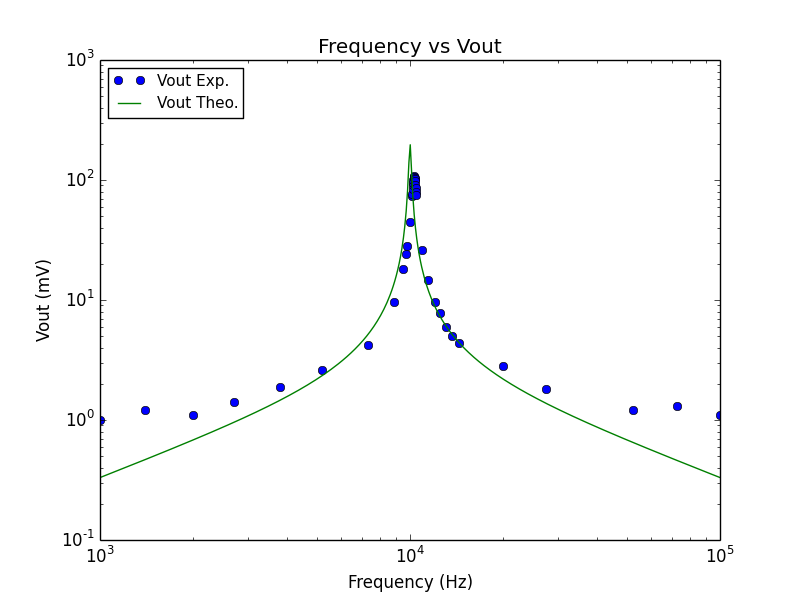
\includegraphics[scale=0.6]{2_6_Q.png}$
    \end{center}
    Now, choosing different load resistances, and we find the following new Q values (Table 3) and compare them with our predicted $Q = R_L \sqrt{\frac{C}{L}}$:
    \begin{table}[h]
    \centering
    \caption{Q-factor with New Load Resistances}
    \label{my-label}
    \begin{tabular}{llllll}
    \textbf{$R_L(\Omega)$} & \textbf{$f_0$(kHz)} & \textbf{$f_1$(kHz)} & \textbf{$f_2$(kHz)} & \textbf{$Q_{exp}$} & \textbf{$Q_{pred}$} \\
    330 & 10.7 & 8.3 & 12.9 & 4.652173913 & 2.011775678 \\
    1000 & 10.26 & 9.5 & 11.2 & 12.07058824 & 6.096289934 \\
    3300 & 10.28 & 10.03 & 10.63 & 34.26666667 & 20.11775678 \\
    10000 & 10.31 & 10.17 & 10.47 & 68.73333333 & 60.96289934 \\
    33000 & 10.31 & 10.23 & 10.4 & 121.2941176 & 201.1775678 \\
    100000 & 10.31 & 10.24 & 10.4 & 128.875 & 609.6289934 \\
     &  &  &  &  &  \\
    \textbf{$R_{ideal}(\Omega)$} & \textbf{$R_{measured}(\Omega)$} &  &  &  &  \\
    330 & 335 &  &  &  &  \\
    1k & 975 &  &  &  &  \\
    3.3k & 3.36k &  &  &  &  \\
    10k & 10.36k &  &  &  &  \\
    33k & 33.96k &  &  &  &  \\
    100k & 100.3k &  &  &  & 
    \end{tabular}
    \end{table}
    The rolloff points are labeled $f_1$ and $f_2$. Plotting the experimental and predicted Q's vs load resistances:\\
    \begin{center}
    $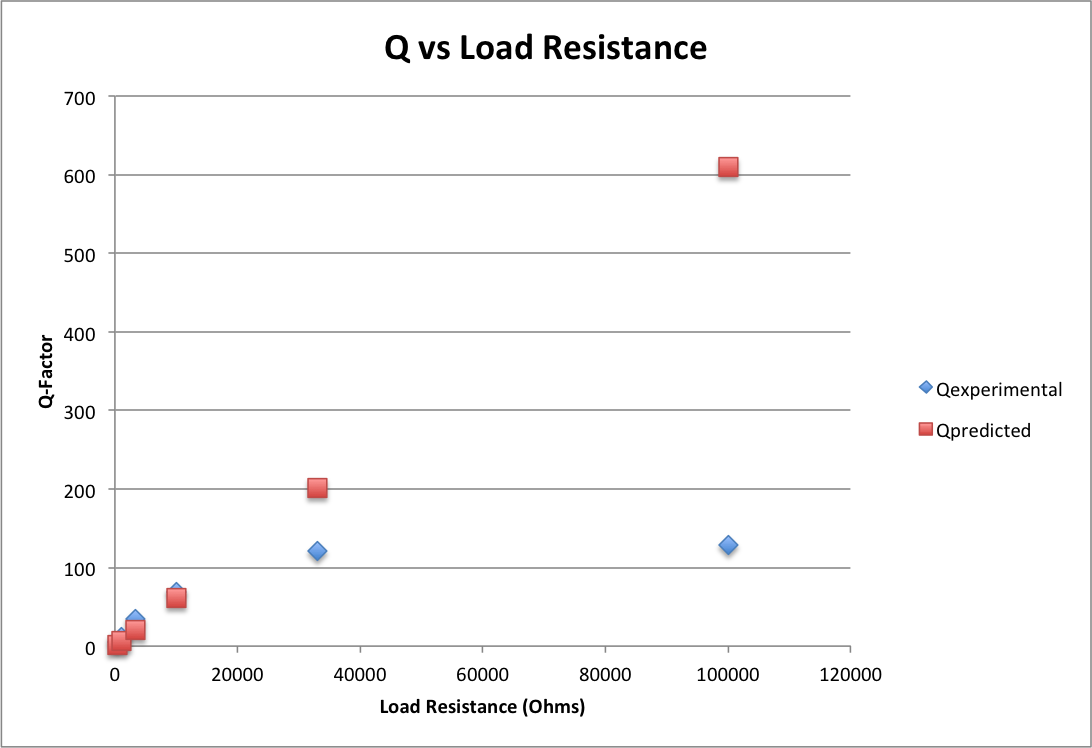
\includegraphics[scale=0.6]{QvsLoad.png}$
    \end{center}
    And we notice that the predicted Qs increase in linear fashion while the experimental Q's begin to asymptote as $R_L \rightarrow \infty$. The curves agree at values below and at 10k$\Omega$ loads, but diverge at higher values. These discrepancies arise from a particular definition of Q, that it is proportional to the energy stored in the oscillator and inversely proportional to the energy dissipated. The predicted Qs continue to increase because it is assumed that as the load resistance increases, more energy is stored in the oscillator and less energy is dissipated in the circuit. However, in all actuality, there are many sources of power loss in the circuit, and we would expect some of the energy stored in the oscillators to dissipate, which would cause Q to decrease. As such, we would expect that the measured Qs would be less than and further diverge from the predicted Qs as the load resistance increases due to additional sources of power loss.


\subsection{Transformer}
    For a 5:25 Step Up Transformer, we would expect the voltage ratio to be:
    \begin{equation}
        \frac{V_2}{V_1} = \frac{N_2}{N_1} = \frac{25}{5} = 5
    \end{equation}
    Where the $_1$ subscript indicates the primary coils and $_2$ indicates the secondary coils. N is the number of turns in the coil.
    For a 25:5 Step Down Transformer, we would expect the voltage ratio to be:
    \begin{equation}
        \frac{V_2}{V_1} = \frac{I_1}{I_2} = \frac{N_2}{N_1} = \frac{5}{25} = 0.2
    \end{equation}
    We define our experimental error to be:
    \begin{equation}
        Error = |\frac{Ratio_{observed}-Ratio_{expected}}{Ratio_{expected}}|*100\%
    \end{equation}
    
    The 20$\Omega$ resistor ($R_1$) measures 20.91 $\Omega$.
    Using $V_{in} = 5V$:\\\indent For the 5:25 Step Up Transformer, $V_{ratio} = \frac{V_2}{V_1} = \frac{17.6V}{4.08V} \approx 4.31$, yielding a relative error of 13.8\%. The result of the step up agrees for the most part; the error were likely associated with how the wires were wrapped around the magnet and how the magnetic fields differed in real life as well as possible sources of power loss. \\\indent For the 25:5 unloaded Step Down Transformer, $V_{ratio} = \frac{V_2}{V_1} = \frac{1.16V}{4.88V} \approx 0.2377$, yielding an error of 18.8\%. There is a little less agreement here, but it is important to note that the voltage clearly stepped down in this case and the absolute error was minimal. \\\indent Increasing $V_{in}$ to 20V, and we find that for the 25:5 unloaded Step Down Transformer, $V_{ratio} = \frac{V_2}{V_1} = \frac{4.6V}{20V} \approx 0.23$, yielding an error of 15\%. The results appear to have some agreement with predictions. \\\indent Adding a loaded resistor of 3 $\Omega$, measured to be $R_2 = 3.49\Omega$ to load the 5-turn output, and we find that for the 25:5 unloaded Step Down Transformer, $V_{ratio} = \frac{2.16V}{9.8V} \approx 0.22$, yielding an error of 10\%. There is much more agreement between expected and measured values in this setup. \\\indent For the last part of this section, we measured the voltage drop across $R_1$, $V_{R1} = 2.861V$ and the voltage drop across $R_2$, $V_{R2} = 2.16V$. Due to the transformer power relation:
    \begin{equation}
        P_1 = I_1 V_1 = I_2 V_2 = P_2
    \end{equation}
    We find that the voltage ratio for the step down transformer of 0.2 should equal the ratio $\frac{I_1}{I_2}$. $I_1 = \frac{V_{R1}}{R_1} = \frac{2.861V}{20.91V} \approx 0.143A$ and $I_2 = \frac{V_{R2}}{R_2} = \frac{2.16V}{3.49V} \approx 0.62A$. The ratio $\frac{I_1}{I_2} = \frac{0.143A}{0.62A} \approx 0.22$, yielding an error of 10\%. A 10\% relative error demonstrates reasonable agreement between the expected and measured values.\\

\subsection{Multisim Tank Simulations}
    See Signature Page

\subsection{Multisim Transient Simulations}
    We noticed that as the transient response dominates, the response curve looks less exponential.\\\indent
    As we increased the capacitance of the RC circuit, the transient response tended to dominate, and the response curve decreased and died off after some time. From an intuitive standpoint, this is because an increase in capacitance increased the amount of charge necessary to register an increase in voltage by the relation $Q = CV$.\\\indent Decreasing the capacitance allowed the response curve to be dominated by the exponential driving voltage, as the capacitor filled up very fast (low time constant $\tau = RC$).\\\indent Increasing resistance allowed the transient response to dominate, as this increase will decrease the current in the circuit, which means that charge will accumulate on the capacitor at a lower rate, decreasing the response voltage. \\\indent Decreasing the resistance allowed the response curve to be dominated by the exponential driving voltage, as this decrease will increase the current, allowing the capacitor to be filled quickly.

\subsection{Resistive Mock Probe-DC Measurements}
    \begin{itemize}
        \item We have built the mock probe with two resistors in series, each with ideal resistance of 1 $M\Omega$; actual values are 1.00 $M\Omega$ and 1.01 $M\Omega$. 
        \item $V_{in}$ of the mock probe is 26.25V, while $V_{out}$ = 0V. The reason that the two measurements are not the same is because the voltage that came in to the probe (24V power supply) was completely dropped across the resistor.
        \item Having connected the scope to the mock probe and measuring with the DMM, we measure $V_{in}$ of the oscilloscope, which also happens to be the $V_{out}$ of the mock probe, to be $8.126V \pm 0.00138V$, the error found from error equation:
        \begin{equation}
            Err(X,Y) = 0:012\%X+ 0:004\%Y
        \end{equation}
        where X is our measured value and Y is the range of the DMM. The $V_{in}$ of the mock probe was found to be $26.25V \pm 0.00715V$ as measured by the DMM. \\\indent Using the oscilloscope to measure, we measure the $V_{out}$ of the mock probe to be 8.65V. Although the value of the $V_{out}$ of the mock probe measured by the scope does not fall within the uncertainty range of that measured by the DMM, we note that the two seem to roughly correspond with one another. These measurements are different than the last set of measurements because now we register about 8 volts across the scope.\\\indent This is because the impedance inside of the scope has roughly the same magnitude as the resistance of the mock probe, so the set up behaves as a voltage divider which does not register an entire voltage drop to zero across its lower leg. \\\indent When we are measuring different circuit elements, we would expect the internal impedance of the voltmeter (scope or DMM) to approach  $\infty$ for a perfect measurement, but in all practicality, this is not so, so we have closer impedance matching.
    \end{itemize}

\subsection{Resistive Mock Probe-AC Measurements}
    The capacitance of a BNC cable was measured to be 162 pF and will factor into the remaining two parts of this lab. The resistors used for the mock probe were the same two from the last section. Table 4 describes the response of the mock probe to input sine waves of $V_{in} = 10V$ (peak-peak) across multiple frequencies. We use a $V_{max}$ of 3.2V to create the relative transfer function Hr = $\frac{V_{max}}{V_{in}}$. Thus, we find a rolloff point at a frequency of 1.5 k$\Omega$, where $V_{out}$ = 2.26V. 
    \begin{table}[h]
    \centering
    \caption{Mock Probe Response}
    \label{my-label}
    \begin{tabular}{ccc}
    \textbf{f(Hz)} & \textbf{$V_{out}$(V)} & \textbf{Hr=$\frac{V_{max}}{V_{in}}$} \\ \hline
    10 & 3.2 & 1 \\
    20 & 3.2 & 1 \\
    50 & 3.2 & 1 \\
    100 & 3.2 & 1 \\
    200 & 3.2 & 1 \\
    500 & 3.12 & 0.975 \\
    1000 & 2.64 & 0.825 \\
    3000 & 1.36 & 0.425 \\
    10000 & 0.448 & 0.14 \\
    30000 & 0.144 & 0.045 \\
    100000 & 0.031 & 0.0096875 \\
    300000 & 0.013 & 0.0040625 \\
    1000000 & 0.013 & 0.0040625 \\
    1500 & 2.26 & 0.70625
    \end{tabular}
    \end{table}
    The transfer function for the theoretical curve is:
    \begin{equation}
       H(f) = \frac{Z_2}{Z_1 + Z_2} = \frac{\frac{\frac{r}{j\omega C}}{r + \frac{1}{j\omega C}}}{R + \frac{\frac{r}{j\omega C}}{r + \frac{1}{j\omega C}}} = \frac{r}{R(jrC*2\pi f + 1) + r}
    \end{equation}
    where $\omega = 2\pi f$, R is the resistance of the mock probe ($\sim 2M\Omega$), r is the resistance inside the scope, and the resistance r ($\sim 1M\Omega$) is in parallel to capacitance ($C = C_{in scope} + C_{BNC} \approx 173.5 pF$) in the scope (see [1.12], eq.(20)). $Z_1$ is the impedance of the mock probe, $Z_2$ is the impedance of the scope (r$||$C), and together, $Z_1$ and $Z_2$ form a voltage divider.\\ However, because we used the relative transfer function Hr = $\frac{V_{out}}{V_{max}}$ in our experimental data, we define Hr such that $Hr = 3.125 * H(f)$ ($\frac{V_{in}}{V_{max}} = 3.125$). Setting Hr = $\frac{1}{\sqrt{2}}$ and solving for f using a numerical analysis and f = 1500 Hz (measured rolloff) as our testing point to be optimized over many iterations, we find that our numerically computed calculated rolloff point is $f_{rolloff calculated} \approx 1488.4 Hz$, which is very close to the measured value. Below we have a bode plot of the measured and calculated $V_{out}$ versus the frequency:
    \begin{center}
        $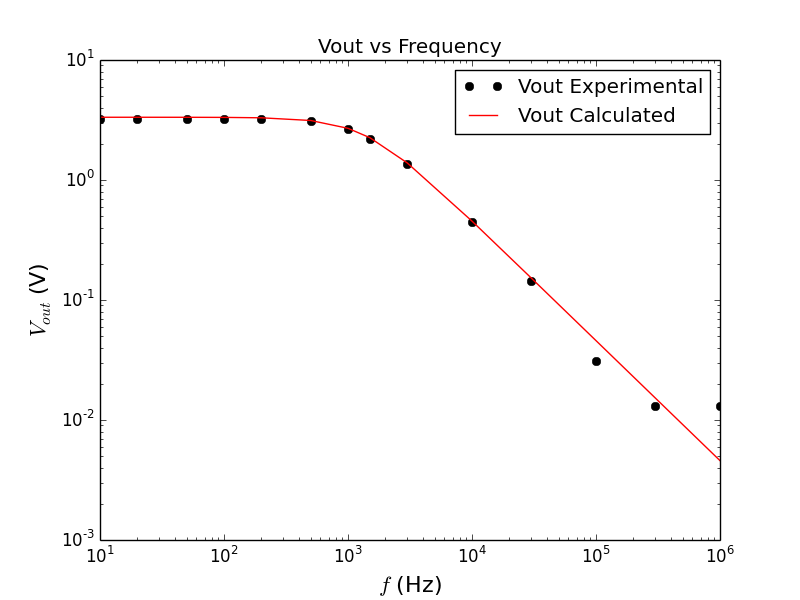
\includegraphics[scale=0.5]{2_11b.png}$
    \end{center}
    \indent From the measured values in Table 4, the plot below, and the bode plot above, we can see that the circuit behaves as a low pass circuit. 
    \begin{center}
    $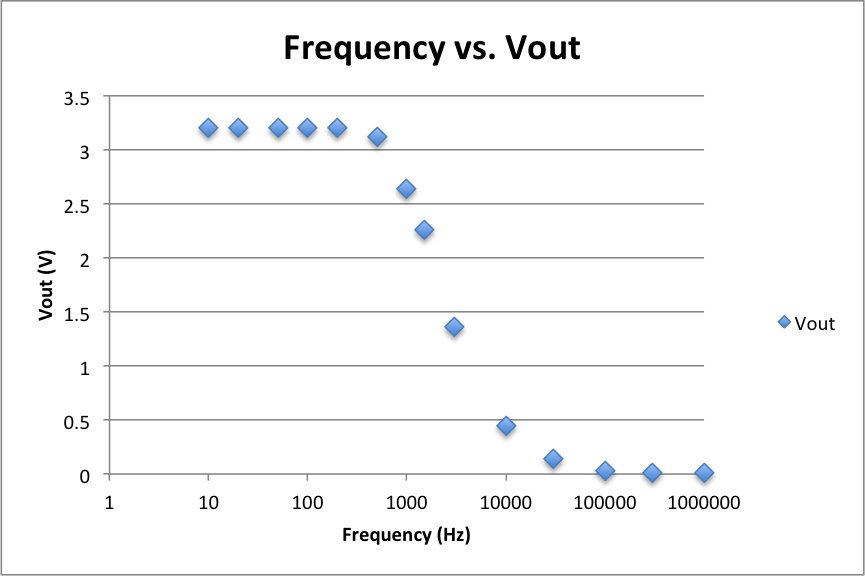
\includegraphics[scale=0.5]{2_11.png}$
    \end{center}
    Here are some typical wave forms for square wave inputs:\\
    \begin{center}
    $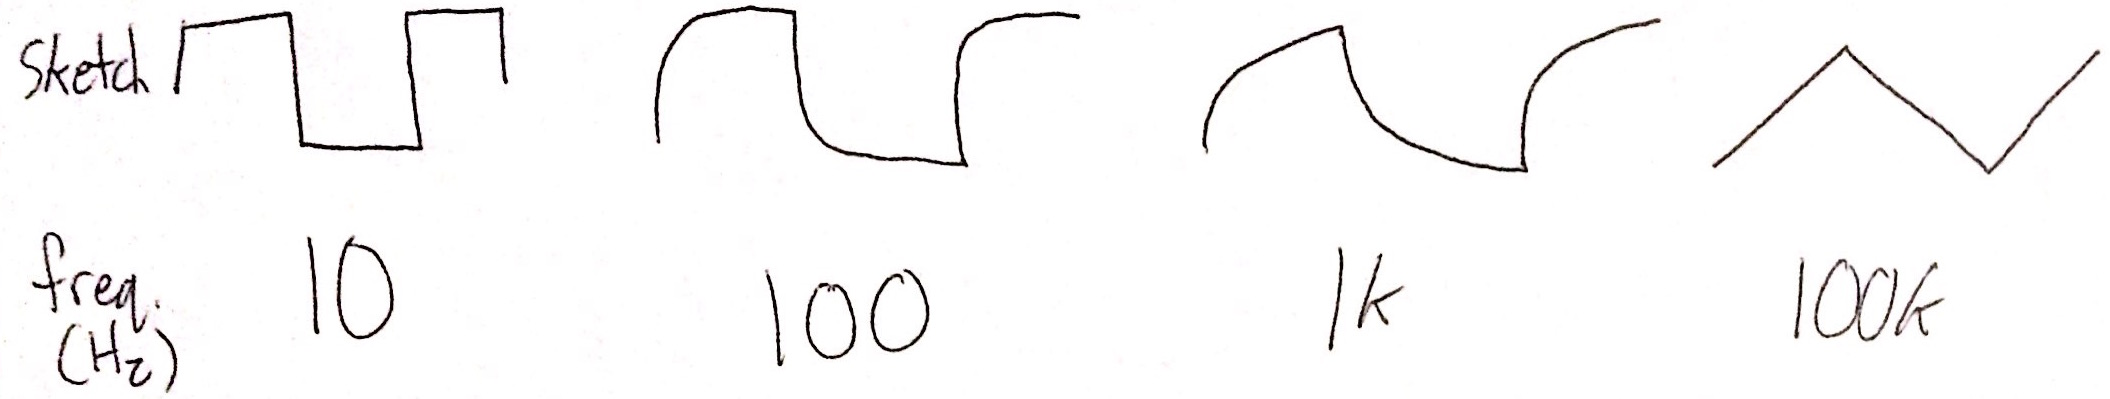
\includegraphics[scale=0.2]{IMG_0184.JPG}$
    \end{center}
    Notice how at high frequencies, we can tell that the output signal behaves as an integrator would.

\subsection{Balanced Mock Probe}
    \indent Building the mock probe for thus section required two series in series, each being 1$M\Omega$. The actual values of the resistors were measured to be 992.3$k\Omega$ and 993.2$k\Omega$. The capacitance we used for our initial "balanced" mock probe was measured to be 19.92 pF, and our input sive wave signal is 10V (peak-peak). \\\indent Scanning the frequency range from 10 Hz to 1 MHz yields the measurements for Table 5, with $V_{max}$ of 3.36V and a rolloff point in the vicinity of the former rolloff point from [1.11]. The circuit still behaves as a low pass circuit, but with $V_{out} \rightarrow 1V$ as $f \rightarrow$ very large values. The initial balanced mock probe with the capacitance of the probe close to 20 pF works slightly better than the mock probe of [1.11], but is still a low pass circuit and produces outputs to square wave input similar to the ones pictured in [1.11]. \\\indent Increasing the value of the capacitor in the mock probe began to reduce the low pass behavior of the circuit. When we used capacitor values that were too high, the circuit began to behave as a high pass filter. The capacitor value that seemed to work best (no filter behavior) was at 82 pF. Any capacitor at a higher value would cause the circuit to behave as a high pass filter, and anything lower would cause the circuit to act as a low pass filter. \\\indent It is possible to remove frequency dependence from the circuit altogether. Suppose we find that the equivalent impedance of the probe is $Z_1$ and the equivalent impedance of the scope is $Z_2$. Our transfer function H is thus:
    \begin{equation}
        H = \frac{V_{out}}{V_{in}} = \frac{Z_2}{Z_1 + Z_2} = \frac{Ae^{j\phi_2}}{Be^{j\phi_b}}
    \end{equation}
    where A, B, $\phi_2$ (phase of $Z_2$), and $\phi_b$ (phase of $Z_1 + Z_2$) are found through the calculation of the transfer function. $e^{j\phi_2} = e^{j\phi_b}$ only if $\phi_1 = \phi_2 = \phi_b$, and in that case, the exponentials in eq.(17) cancel out and the transfer function is no longer frequency dependent. The complex part of each exponential depends on frequency, so if the phases are matched, then the frequency-dependence is eliminated. \\\indent The conditions by which this holds does not require direct calculation of the transfer function; we can separate the probe and the scope into a voltage divider, with the probe being in the upper leg and the scope being in the lower leg. Both components function as independent RC circuits, the time constants of which are:
    \begin{equation}
        \tau_{probe} = R_{probe}*C_{probe}
    \end{equation}
    \begin{equation}
        \tau_{scope} = R_{scope}*C_{scope}
    \end{equation}
    Where $R_{probe}$ equals the sum of the two series resistors as aforementioned, $R_{scope} = 1M\Omega$, and $C_{scope}$ is the equivalent capacitance of the capacitance internal to the scope (11.5 pF) in parallel with the capacitance of the BNC cable (162 pF measured using the LCR meter), which is hooked up in parallel to the scope. The result:
    \begin{equation}
        C_{scope} = C + C_{BNC} = 11.5pF + 162 pF = 173.5 pF
    \end{equation}
    \\\indent the time constants of the upper and lower legs equal to each other and solving for $C_{probe}$ best accomplishes the task of finding the best capacitance value that will remove all frequency dependence of the scope because we would expect the two time constants to be equal when the time it takes for the capacitor in the lower leg to charge is the same time it takes for the capacitor in the upper leg to charge. The capacitors should charge and discharge with the same timing in order to ensure that the driving signal is in phase with the response signal. Thus, supposing $\tau_{probe} = \tau_{scope}$, we can calculate:
    \begin{equation}
        best C_{probe} = \frac{R_{scope}*C_{scope}}{R_{probe}} = \frac{1 M\Omega*173.5 pF}{992.3k + 993.2k} \approx 87.38 pF
    \end{equation}
    This value is very close to the capacitor value that appeared to significantly reduce all filtering effects (82 pF), and with a 20\% capacitance tolerance included in the analysis, the best $C_{probe}$ definitely lies within the uncertainty range of the 82 pF capacitor.
    \begin{table}[]
    \centering
    \caption{Balanced Mock Probe Response}
    \label{my-label}
    \begin{tabular}{ccc}
    \textbf{f(Hz)} & \textbf{$V_{out}$(V)} & \textbf{Hr=$\frac{V_{max}}{V_{in}}$} \\ \hline
    10      & 3.36    & 1           \\
    20      & 3.36    & 1           \\
    50      & 3.36    & 1           \\
    100     & 3.34    & 0.994047619 \\
    200     & 3.3     & 0.982142857 \\
    500     & 3.12    & 0.928571429 \\
    1000    & 2.64    & 0.785714286 \\
    3000    & 1.54    & 0.458333333 \\
    10000   & 1.06    & 0.31547619  \\
    30000   & 1       & 0.297619048 \\
    100000  & 1       & 0.297619048 \\
    300000  & 1       & 0.297619048 \\
    1000000 & 1       & 0.297619048
    \end{tabular}
    \end{table}
    


\section{Signature Page}
\centering
$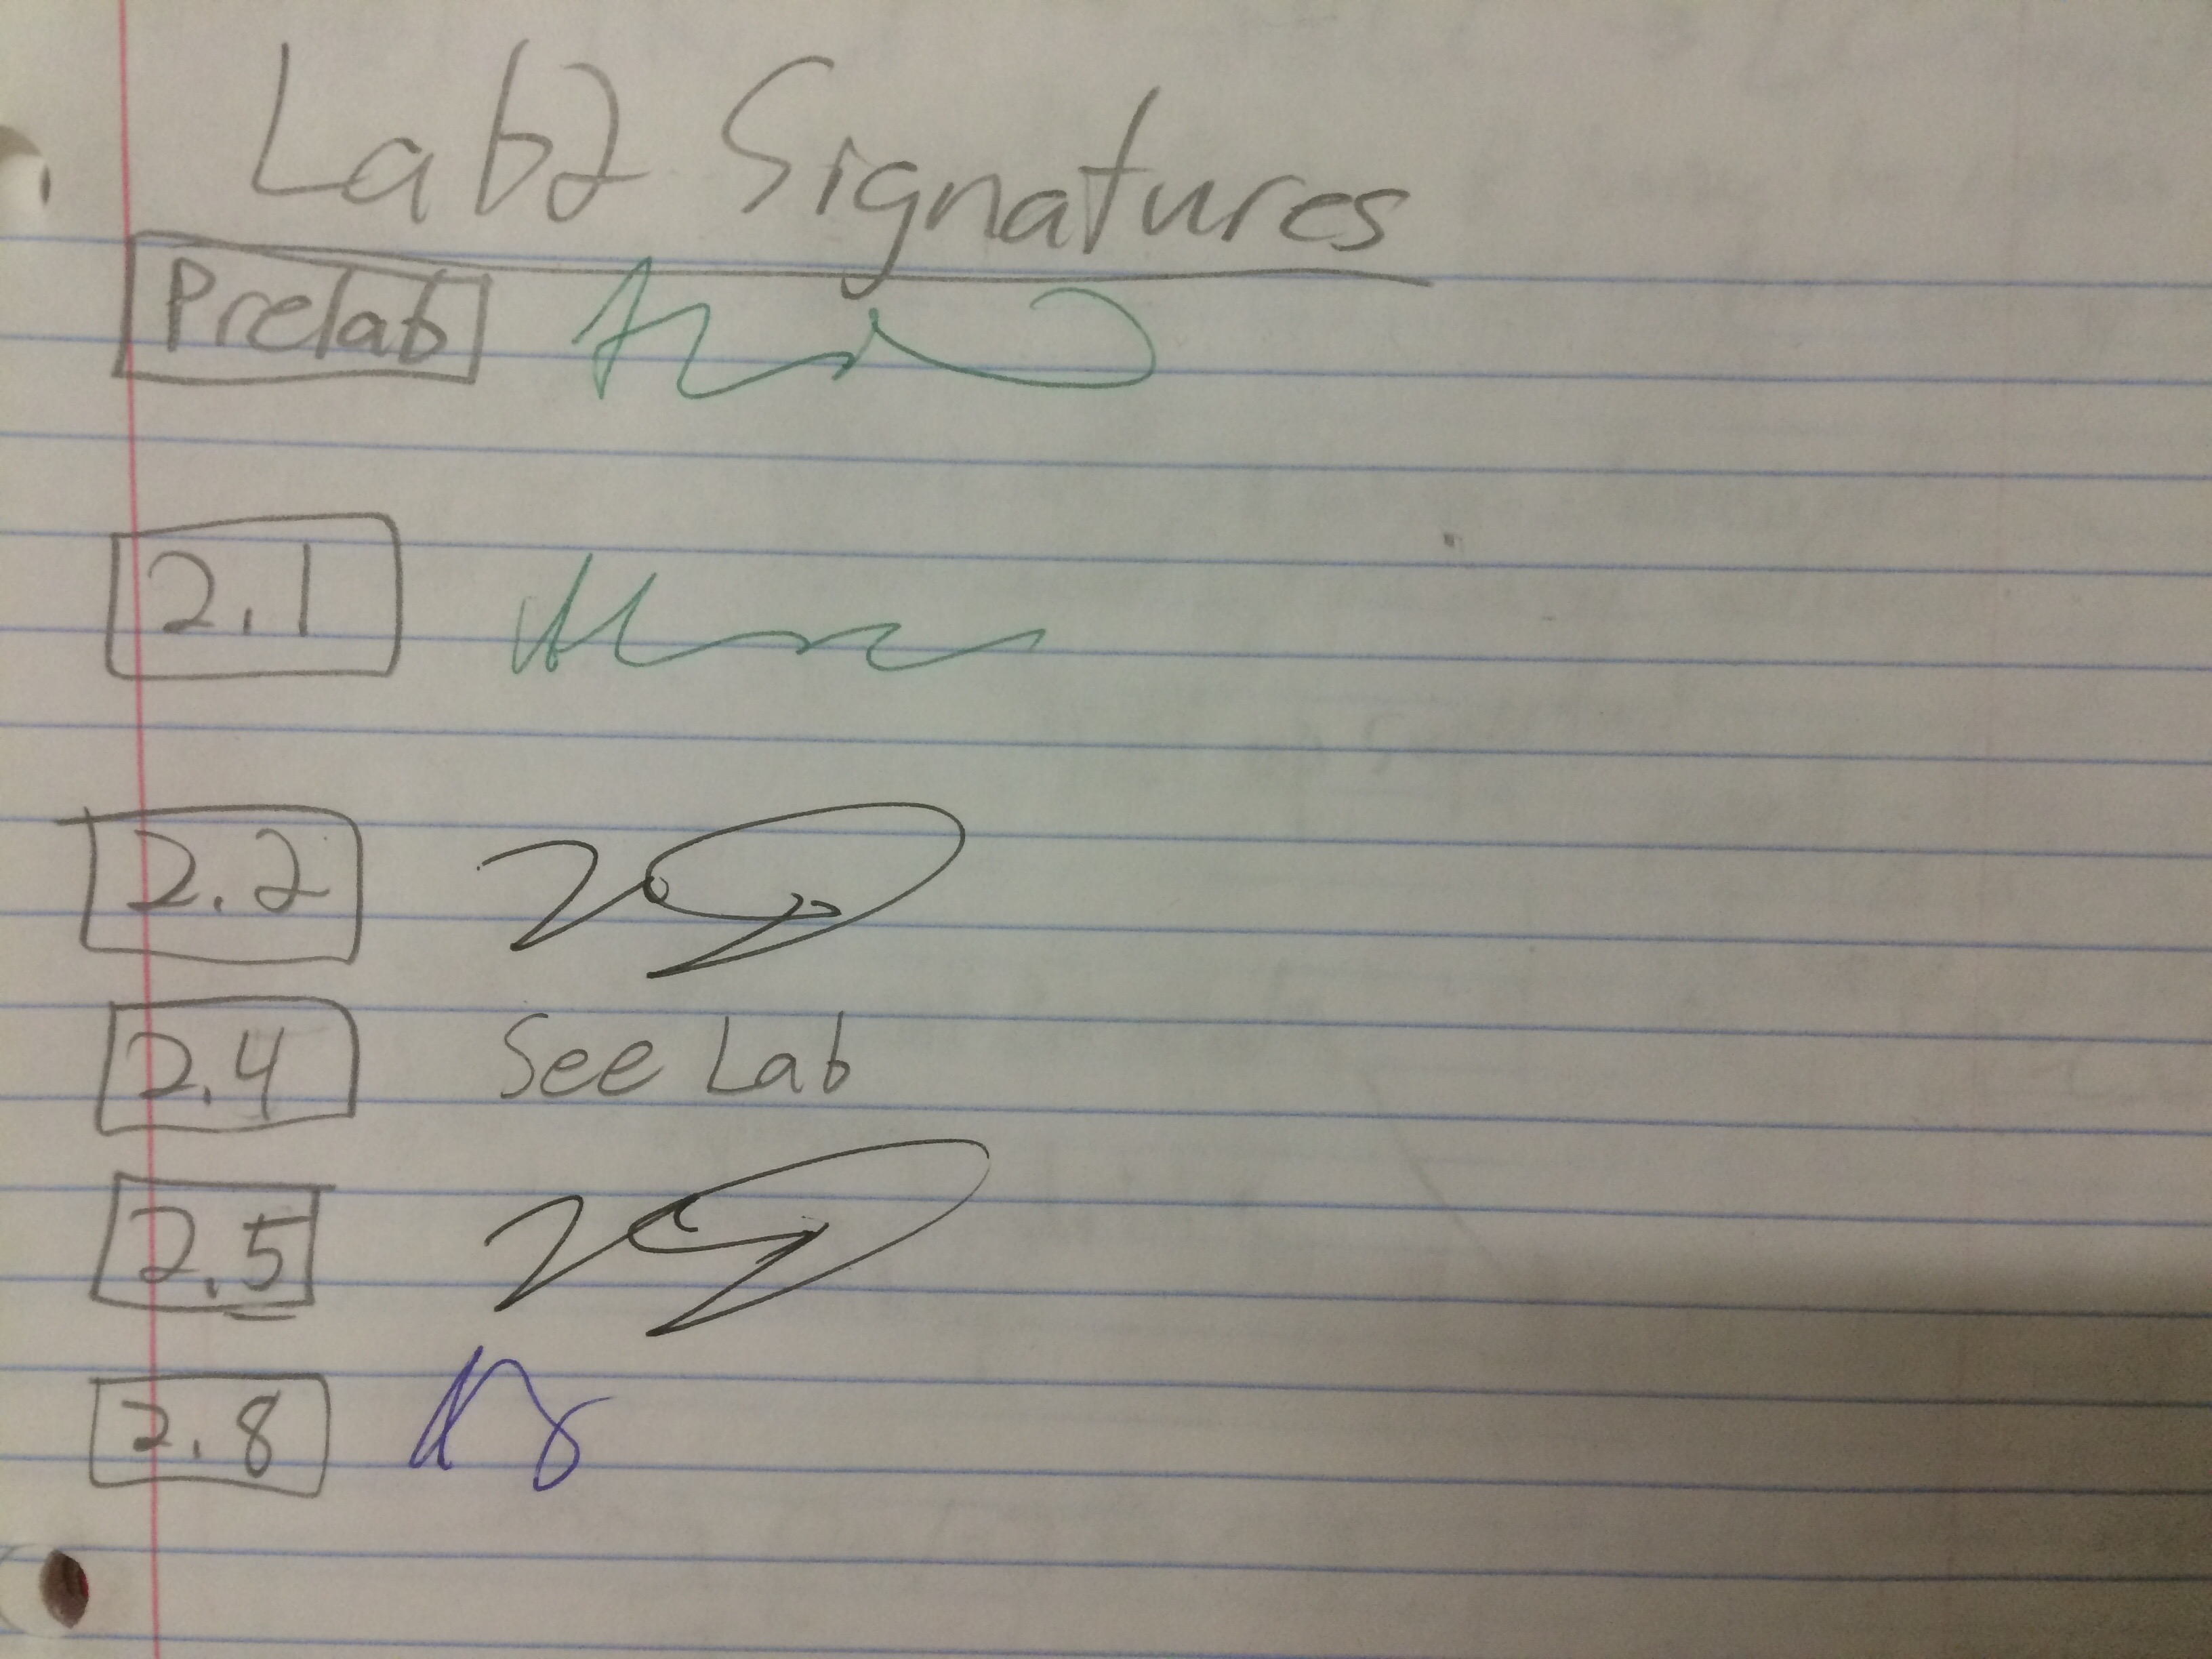
\includegraphics[scale=0.1]{IMG_0170.JPG}$

\bibliographystyle{plain}
\bibliography{joshbib}

\end{document}

